\section{Open-sky conditions}
\label{sec:opensky}
\subsection{Raw measurements - HW clock de-sync}
% To evaluate the quality and consistency of raw GNSS measurements on Android smartphones, we analyzed data collected from a Samsung Galaxy S23 Ultra in Airplane mode, using: \textbf{GNSSLogger} (developed by Google) and \textbf{GPSTest} (an open-source GNSS diagnostic tool). 

% Data collection was carried out in Parco Cavalieri di Vittorio Veneto, located in Torino, Italy, under clear weather conditions. The test device was placed in an open-sky environment, isolated approximately 20 meters from nearby obstructions (fig. \ref{fig:map}), ensuring minimal multipath interference and optimal reception of the GNSS signal. 
% To ensure maximum measurement continuity and stability, all adaptive battery saving features of the operating system were disabled, including background activity restrictions and battery optimization settings for GNSSLogger. This was done to prevent throttling or suspension of GNSS-related processes during data logging.

During our first experiment, which we conducted under all conditions specified in \ref{sec:tools}, we observed hardware clock discontinuities that directly affected the reliability of pseudorange computations.


\begin{figure}[H]
        \centering
        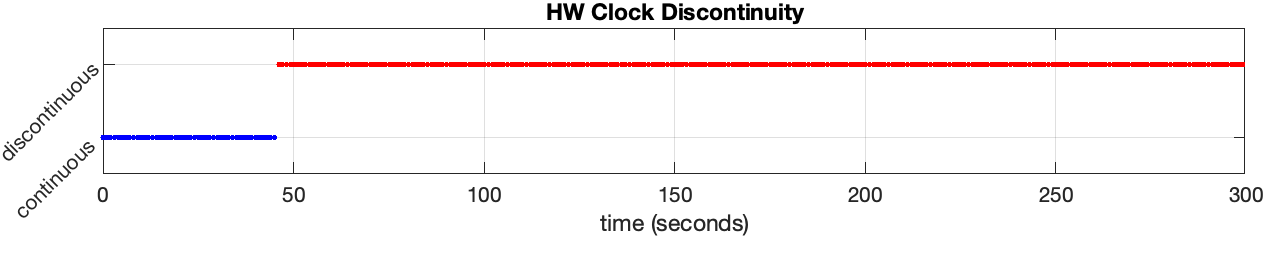
\includegraphics[width=0.85\linewidth]{images/discontinuity_gnss_log.png}
        \caption{Status of GNSS hardware clock over time with just GNSSLogger}
        \label{fig:GNSSLogger-discontinuity}
\end{figure}

Although no power-saving modes of any kind were active in the mobile device, HW clock discontinuities, indicated by a transition from blue (continuous) to red (discontinuous), were detected at approximately 46 seconds into the logging session and persisted for the duration of the test (fig. \ref{fig:GNSSLogger-discontinuity}).
This discontinuity indicates that the device’s internal clock experienced a sudden and irregular change in its progression. Instead of increasing smoothly over time, the clock may have jumped forward, backward, or altered its rate. This issue is not caused by a loss of synchronization with GNSS time, which is always managed through a clock bias, but rather by a sudden instability in the internal device clock that breaks the assumption of consistent bias over time. As a result, time-dependent computations, such as speed estimation or pseudorange rate, become unreliable from the point of discontinuity onward.

% \colorbox{red}{https://sites.google.com/view/gnsstutorial}
\begin{figure}[H]
    \centering
    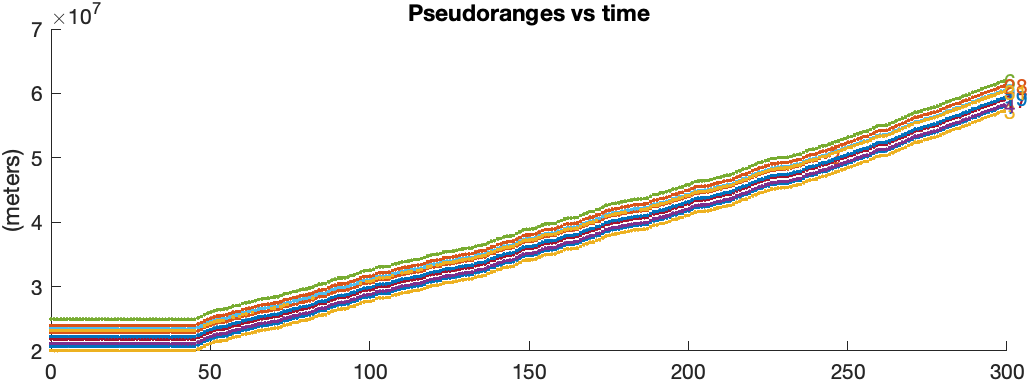
\includegraphics[width=0.75\linewidth]{images/disontinuity_pseudorange_vs_time.png}
    \caption{Pseudoranges vs. time under HW clock discontinuity}
    \label{fig:disontinuity_pseudorange_vs_time}
\end{figure}

As shown in Figure \ref{fig:disontinuity_pseudorange_vs_time}, after the clock discontinuity occurs, all pseudorange values begin to increase steadily and appear very similar across all satellites. This unusual pattern is caused by an incorrect handling of the clock bias during the computation of the GNSS receive time (\textit{tRxNanos}).

In the script, \textit{tRxNanos} is calculated using the expression:
\begin{equation*}
    \label{eq:tRxNanos}
    \text{tRxNanos} = \text{TimeNanos} - \text{FullBiasNanos}(1) - \text{weekNumberNanos}
\end{equation*}
where \textit{TimeNanos} is the internal time of the device at the moment of signal reception, \textit{FullBiasNanos} is the correction term that accounts for the difference between the device’s clock and true GNSS time, and \textit{weekNumberNanos} adjusts for GPS week rollovers.

However, the script applies a constant \textit{FullBiasNanos} value across the entire dataset, using the one extracted from the first epoch (\textit{FullBiasNanos(1)}). In reality, the clock bias is not constant: it can drift over time or change abruptly in the presence of a clock discontinuity. When this happens, \textit{TimeNanos} may suddenly jump, but since the bias is not updated accordingly, it no longer compensates correctly. This causes \textit{tRxNanos} to become inaccurate from that point on, introducing a common shift in the receive time for all satellites.
This has a significant effect on the pseudorange calculation, which is defined as:
\begin{equation*}
    \text{pseudorange} = (tRx - tTx)c
\end{equation*}
where \textit{tRx} is the receiver time computed as \ref{eq:tRxNanos}, \textit{tTx} is the transmission time from the satellite and \textit{c} is the speed of light.
When the signals from the satellites arrive at the same time, \textit{tRx} will be identical for all of them. In this case, the differences in the pseudoranges are determined solely by the \textit{tTx}, the timestamp of each satellite’s signal transmission. However, even a small error in \textit{tRx}, in the order of microseconds (as showed in \ref{fig:discontinuity_bias_clock}), can result in a large pseudorange error because it is multiplied by the speed of light. As a result, the pseudoranges may appear almost identical in the graph due to this large error, which grows over time.

Despite these errors in PR computation, the estimated positions remain approximately correct. This is because the weighted least squares solution simultaneously estimates not only the receiver’s position and velocity but also the clock bias as an unknown parameter. As a result, even if the initial bias used in the pseudorange computation is outdated or incorrect, the solver adjusts the bias dynamically during the estimation process. However, since the initial PR inputs are distorted by the uncorrected bias, the system starts from less precise measurements, which can slightly degrade the accuracy of the estimated position and velocity (fig. \ref{fig:discontinuity_map_computed_position_vs_true_postion}).

\begin{figure}[H]
    \centering
    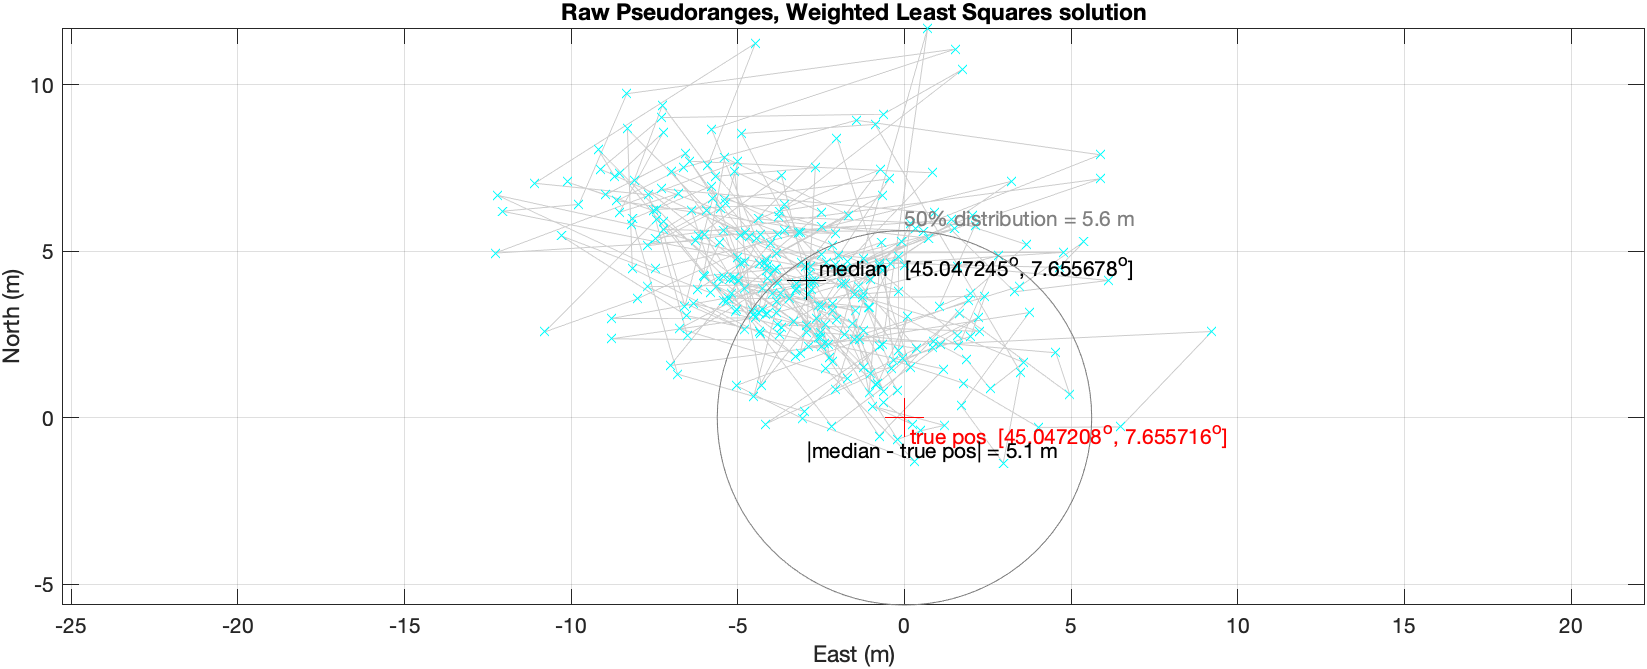
\includegraphics[width=0.85\linewidth]{images/discontinuity_map_computed_position_vs_true_postion.png}
    \caption{Computed position with discontinuity clock vs true position}
    \label{fig:discontinuity_map_computed_position_vs_true_postion}
\end{figure}

\subsubsection{Solving the HW clock discontinuity}
 
While the WLS algorithm partially compensates for bias errors, a better solution was found by directly preventing the discontinuities from occurring.
In particular, launching the GPSTest \cite{gpsTestApp} app in parallel with GNSSLogger during data collection sessions eliminated HW clock discontinuities (fig. \ref{fig:GNSSLogger-continuity}). 

% As shown in fig. \ref{fig:GNSSLogger-continuity}, the hardware clock remained continuous for the full duration of the experiment.
This behavior suggests that the root cause is not related to external environmental factors, but rather stems from the internal management of GNSS resources on the Android platform, like foreground priority and wake locks, leading to clock resets or timing irregularities.
By forcing continuous GNSS activity through GPSTest, this behavior is suppressed entirely, and the hardware clock remains stable throughout the session.

In order to obtain better results, without discontinuity, all subsequent surveys were carried out using the two applications, GNSSLogger and GPSTest, run in parallel.


\subsection{Raw measurements - no HW clock de-sync}
Having solved the HW clock de-synchronization issue, the logging produced the best samples we had, which we will use as a baseline to analyze worse scenarios. Correlating the logs with the visibility skyplot produced by the MATLAB notebook \cite{skyplotsNotebook} (fig. \ref{fig:skyplot_punto_3}), we can see how the phone's receiver has been continuously able to receive signals from all visible satellites, except for satellites 20, 26 and 30, which were possibly out of sight because of their low elevation angle of less than 10 degrees above the horizon. In addition, HDOP has been stable at a value of 0.8 (fig. \ref{fig:hdop_punto_3}), which indicates very good geometrical conditions.

The C/N0 plot (fig. \ref{fig:CN0_punto_3}) shows how the intensities of signals from visible satellites have no immediate correlation with the elevation angle; in particular, we see how satellites closer to our Zenith and closer in terms of straight-line distance, as shown by the pseudoranges (fig. \ref{fig:pseudoranges_opensky}), are not among the strongest signals we received. Finally, some signals were surely more stable in their intensity than others; examples of this behavior are satellite 4 (very stable at more than 50 dB-Hz) and satellite 7 (oscillating in a range between 30 and 45 dB-Hz).

\begin{figure}[H]
    \centering
    \begin{minipage}[b]{0.40\linewidth}
        \centering
        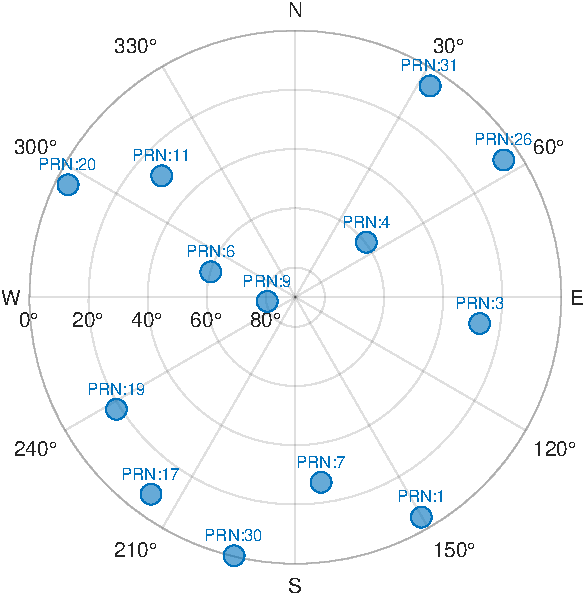
\includegraphics[width=\linewidth]{images/skyplot_punto_3.pdf}
        \caption{Skyplot of visible satellites at 20:16:32 UTC+2}
        \label{fig:skyplot_punto_3}
    \end{minipage}
    \hfill
    \begin{minipage}[b]{0.56\linewidth}
        \centering
        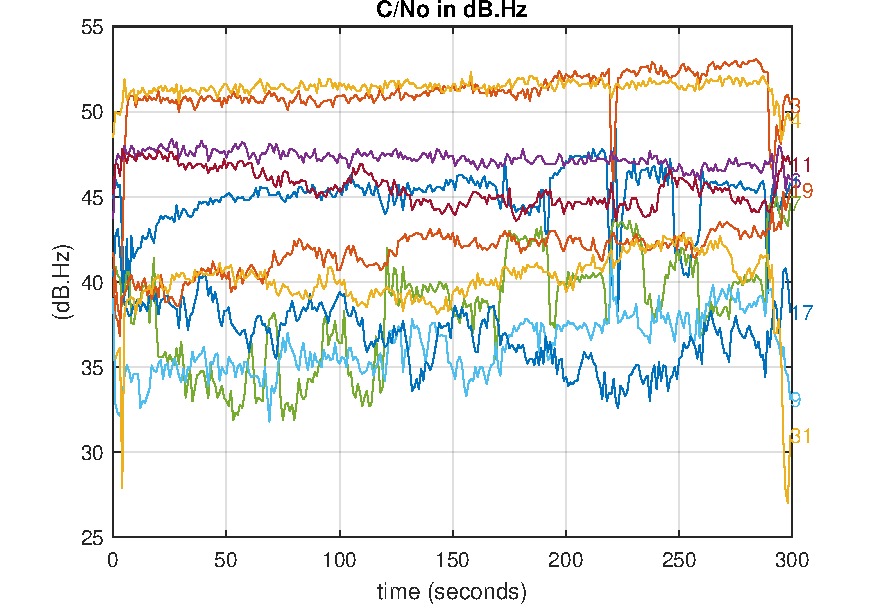
\includegraphics[width=\linewidth]{images/CN0_punto_3.pdf}
        \caption{Carrier to noise density ratio, dB-Hz}
        \label{fig:CN0_punto_3}
    \end{minipage}
\end{figure}

\subsection{Position, Velocity and Time}
The open-sky conditions are also reflected in the quality of the results obtained in terms of position, velocity and time estimation. We obtained very stable results; the 50\% computed positions were within a circle of radius of 1 m (fig. \ref{fig:pos_punto_3_precision}), with an error of 5.4 meters between the median and the real position (on the horizontal plane) (fig. \ref{fig:pos_punto_3}). 

However, comparing the estimated altitude with the actual one (obtained via Google Earth), we observed a significant discrepancy, not only due to the precision of the GNSS system, but also to the difference in models used to represent the shape of the Earth \cite{esriGeoidArticle} \cite{eosElevation2025}. In particular, Google Earth uses the EGM96 geoidal model for the planet \citep{googleEarthModel} \citep{googleEarthModel2}, and therefore refers to an orthometric height, while the script we used relies on the WGS84 ellipsoid model, and outputs an ellipsoid height. The geoid height for the specific location is easily retrieved by using online tools \cite{geoidHeightCalculator}. 

% ellipsoid is lower than geoid, like in our case. If changing this, change it to something similar.
\begin{figure}[H]
    \centering
    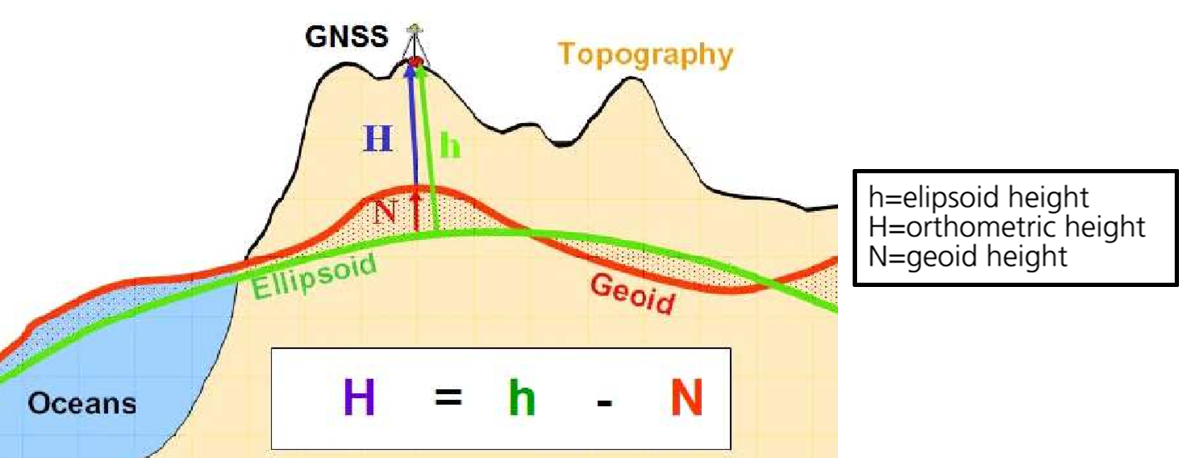
\includegraphics[width=0.50
    \linewidth]{images/geoidellipsoid_legenda.png}
    \caption{Orthometric and ellipsoid height, taken from \cite{kaminskis2008quasigeoid}.}
    \label{fig:h=H+N}
\end{figure}

In our case, the median altitude  reported by the MATLAB tool ($h$) was 321 m, the one obtained from Google Earth ($H$) was 250 m and the geoid height in our location ($N$) is 48 m, so the error in the altitude estimation is $h - (H + N) = (321 - 250 - 48)\ \SI{}{\meter}= \SI{23}{\meter}$, which aligns with our expectations about the vertical accuracy \cite{Enge2010-uj}.



% This leads to an altitude difference that is measured by subtracting the geoid height from the ellipsoid height - equivalently, it's the difference between orthometric height and geoid height at the location being evaluated (which is easily retrieved by using online tools \cite{geoidHeightCalculator}) \cite{esriGeoidArticle}. 


